\documentclass[USenglish]{article}
\usepackage[utf8]{inputenc}
\usepackage[T1]{url}

\usepackage[a4paper]{geometry}
\usepackage{listings}

\setlength{\parskip}{1em}
\setlength{\parindent}{0em}
\usepackage{caption}
\usepackage{subcaption}

\urlstyle{sf}

\usepackage[table]{xcolor}
\usepackage{tikz,babel,textcomp,csquotes,varioref,graphicx,float}
\usepackage{tikz-uml}
\usepackage{babel}
\usepackage{graphicx}
\usepackage{ifikompendiumforside}
\usepackage{hyperref}
\usepackage{array}
\usepackage[font={small,it,sf}]{caption}
\usepackage{longtable}
\usepackage{multirow}
\usepackage{wrapfig}
\usepackage{titlesec,titletoc}
\usetikzlibrary{arrows, shadows}

\newcommand{\TRUE}{\cellcolor{green}{\textbf{True}}}
\newcommand{\YES}{\cellcolor{green}{\textbf{Yes}}}
\newcommand{\FALSE}{\cellcolor{red}{\textbf{False}}}
\newcommand{\NO}{\cellcolor{red}{\textbf{No}}}
\newcommand{\NONE}{\cellcolor{gray}{\textbf{--}}}

\title{INF4121 Project Assignment 2}
\subtitle{Testing and test automation}
\author{Per Øyvind Karlsen}

\begin{document}
\ififorside

\section{Introducion}

\subsection{Objective}

\section{Requirement 1}

\subsection{Manual tests}

\subsubsection{1. Register new customer, login, password reset}

\paragraph{Register new customer \& login}

\begin{table}[ht]
\centering
\caption{Decission table}
\label{newuser-decission-table}
\begin{tabular}{|c|l|c|c|c|c|}
\hline
\parbox[t]{3mm}{\multirow{4}{*}{\rotatebox[origin=c]{90}{Conditions}}} &
New user 		& \TRUE	& \FALSE	& \FALSE	& \NONE		\\ \cline{2-6} &
Valid username		& \NONE	& \FALSE	& \NONE		& \TRUE		\\ \cline{2-6} &
Valid password		& \NONE	& \NONE		& \FALSE	& \TRUE		\\ \cline{2-6} &
\multicolumn{5}{l|}{} \\
\hline
\parbox[t]{3mm}{\multirow{3}{*}{\rotatebox[origin=c]{90}{Actions}}} &
Create user		& \YES	& \NO		& \NO		& \NO		\\ \cline{2-6} &
Login fail (error) 	& \NO	& \YES		& \YES		& \NO		\\ \cline{2-6} &
Login success		& \YES	& \NO		& \NO		& \YES		\\ \hline
\end{tabular}
\end{table}

\paragraph{Register new customer}

\begin{table}[ht]
\centering
\caption{Use case}
\label{newuser-use-case}
\begin{tabular}{|l|l|p{8cm}|}
\hline
\multirow{6}{*}{\begin{tabular}[l]{@{}l@{}}\\ \\ \\ Main Success Scenario\\ A: Actor	\\ S: System	\end{tabular}} &
Step	&	Description 					\\ \cline{2-3} &
1	&	A: Open the e-commerce website   		\\ \cline{2-3} &
2	&	A: Click "Sign In"				\\ \cline{2-3} &
4	&	A: Click "REGISTER" button			\\ \cline{2-3} &
5	&	A: Enter valid email address \& password, remaining fields optional	\\ \cline{2-3} &
6	&	A: Click "REGISTER" button			\\ \cline{2-3} &
7	&	S: Validate new user information 		\\ \cline{2-3} &
8	&	S: Create user account				\\ \cline{2-3} &
9	&	S: Authenticate user				\\ \cline{2-3}
\hline
\multirow{3}{*}{Extensions} &
7a	&	\begin{tabular}[c]{@{}l@{}}
		Username/email address invalid/missing \\
		S:Display proper error message
		\end{tabular}	\\ \cline{2-3} &
7b	&	\begin{tabular}[c]{@{}l@{}}
		Password missing or mismatch \\
		S:Display proper error message
		\end{tabular}	\\ \cline{2-3}
\hline
\end{tabular}
\end{table}

\paragraph{Login}

\begin{table}[ht]
\centering
\caption{Use case}
\label{login-use-case}
\begin{tabular}{|l|l|p{8cm}|}
\hline
Preconditions:	& \multicolumn{2}{l|}{User exists and is logged out} \\ \hline
\multirow{6}{*}{\begin{tabular}[l]{@{}l@{}}\\ \\ \\ Main Success Scenario\\ A: Actor	\\ S: System	\end{tabular}} &
Step	&	Description 					\\ \cline{2-3} &
1	&	A: Open the e-commerce website   		\\ \cline{2-3} &
2	&	A: Click "Sign In"				\\ \cline{2-3} &
3	&	A: Enter user email address \& password		\\ \cline{2-3} &
4	&	A: Click "SIGN IN" button			\\ \cline{2-3} &
5	&	S: Authenticate user				\\ \cline{2-3}
\hline
\multirow{3}{*}{Extensions} &
5a	&	\begin{tabular}[c]{@{}l@{}}
		Invalid e-mail \\
		S:Display proper error message
		\end{tabular}	\\ \cline{2-3} &
5b	&	\begin{tabular}[c]{@{}l@{}}
		Valid e-mail and incorrect password \\
		S:Display proper error message
		\end{tabular}	\\ \cline{2-3}
\hline
\end{tabular}
\end{table}


\paragraph{Password reset}

\begin{table}[ht]
\centering
\caption{Use case}
\label{change-password-use-case}
\begin{tabular}{|l|l|l|}
\hline
Preconditions:	& \multicolumn{2}{l|}{User logged in} \\ \hline
\multirow{6}{*}{\begin{tabular}[l]{@{}l@{}}\\ \\ \\ Main Success Scenario\\ A: Actor	\\ S: System	\end{tabular}} &
Step	&	Description 					\\ \cline{2-3} &
1	&	A: Click "Change Password"	   		\\ \cline{2-3} &
2	&	A: Enter current password, new password and retype password	\\ \cline{2-3} &
3	&	A: Click "CONTINUE" button			\\ \cline{2-3} &
4	&	S: Validate Passwords				\\ \cline{2-3} &
5	&	S: Change password				\\ \cline{2-3} &
7	&	A: Click "Sign Out"				\\ \cline{2-3} &
8	&	A: Enter username \& new password		\\ \cline{2-3} &
9	&	A: Click "SIGN IN" button			\\ \cline{2-3} &
10	&	S: Authenticate user				\\ \cline{2-3}
\hline
\multirow{3}{*}{Extensions} &
4a	&	\begin{tabular}[c]{@{}l@{}}
		Invalid current password incorrect and valid new password combination \\
		S:Display proper error message
		\end{tabular}	\\ \cline{2-3} &
4b	&	\begin{tabular}[c]{@{}l@{}}
		Valid current password and invalid new password combination \\
		S:Display proper error message
		\end{tabular}	\\ \cline{2-3}
\hline
\end{tabular}
\end{table}

\subsubsection{Selecting products}

\begin{table}[ht]
\centering
\caption{Use case}
\label{selecting-products-use-case}
\begin{tabular}{|l|l|l|}
\hline
Preconditions:	& \multicolumn{2}{l|}{User logged in with cart empty} \\ \hline
\multirow{3}{*}{\begin{tabular}[l]{@{}l@{}}Main Success Scenario\\ A: Actor	\\ S: System	\end{tabular}} &
Step	&	Description 						\\ \cline{2-3} &
1	&	A: Click "ADD TO CART" for a product in the store	\\ \cline{2-3} &
2	&	S: Add product to cart					\\ \cline{2-3}
\hline
\end{tabular}
\end{table}

\subsubsection{Continue Shopping}

\begin{tikzpicture}[scale=0.5, transform shape]
	\begin{umlstate}[name=continueShopping]{Continue shopping}
		\umlstateinitial[x=4, name=addProduct]
		\umlbasicstate[x=4, y=-3, name=shoppingCart, fill=white]{Shopping cart}
		\umlHVtrans[arg={User adds product}, pos=1.2]{addProduct}{shoppingCart}

		\umlbasicstate[y=-6, name=increaseQuantity, fill=white, scale=0.5]{Increase Quantity}
		\umltrans{shoppingCart}{increaseQuantity}

		\umlbasicstate[x=8, y=-6, name=addNewItem, fill=white]{Add New Item}
		\umltrans{shoppingCart}{addNewItem}

		\umlbasicstate[x=4, y=-9, name=updateItems, fill=white]{Update total number of items}
		\umltrans{increaseQuantity}{updateItems}
		\umltrans{addNewItem}{updateItems}

		\umlstateexit[x=4, y=-12, name=productAdded, fill=black, color=white]{Product added}

		\umltrans[arg={Products updated}, pos=1]{updateItems}{productAdded}
	\end{umlstate}
\end{tikzpicture}

\begin{table}[ht]
\centering
\caption{Use case}
\label{continue-shopping-use-case}
\begin{tabular}{|l|l|l|}
\hline
Preconditions:	& \multicolumn{2}{l|}{User logged in with one item in cart} \\ \hline
\multirow{6}{*}{\begin{tabular}[l]{@{}l@{}}\\ \\ \\ Main Success Scenario\\ A: Actor	\\ S: System	\end{tabular}} &
Step	&	Description 						\\ \cline{2-3} &
1	&	A: Click "ADD TO CART" for another product in the store	\\ \cline{2-3} &
2	&	S: Add product to cart					\\ \cline{2-3} &
\hline
\end{tabular}
\end{table}

\subsubsection{Checkout}

\begin{table}[ht]
\centering
\caption{Use case}
\label{checkout-use-case}
\begin{tabular}{|l|l|l|}
\hline
Preconditions:	& \multicolumn{2}{l|}{User logged in with items in cart} \\ \hline
\multirow{6}{*}{\begin{tabular}[l]{@{}l@{}}\\ \\ \\ Main Success Scenario\\ A: Actor	\\ S: System	\end{tabular}} &
Step	&	Description 					\\ \cline{2-3} &
1	&	A: Click "Checkout"		   		\\ \cline{2-3} &
2	&	A: Click "Continue Checkout"			\\ \cline{2-3} &
3	&	A: Fill out form				\\ \cline{2-3} &
4	&	A: Click "Continue Checkout"			\\ \cline{2-3} &
5	&	A: Select shipping method			\\ \cline{2-3} &
5	&	A: Click "Continue Checkout"			\\ \cline{2-3} &
6	&	S: Validate shipping method			\\ \cline{2-3}
\hline
\multirow{1}{*}{Extensions} &
6a	&	\begin{tabular}[c]{@{}l@{}}
		Shipping option not selected \\
		S:Display proper error message
		\end{tabular}	\\ \cline{2-3}
\hline
\end{tabular}
\end{table}

\subsubsection{Change number of items}

\begin{table}[ht]
\centering
\caption{Use case}
\label{change-number-of-items-use-case}
\begin{tabular}{|l|l|l|}
\hline
Preconditions:	& \multicolumn{2}{l|}{User logged in with items in cart} \\ \hline
\multirow{6}{*}{\begin{tabular}[l]{@{}l@{}}\\ \\ \\ Main Success Scenario\\ A: Actor	\\ S: System	\end{tabular}} &
Step	&	Description 						\\ \cline{2-3} &
1	&	A: Click on "My cart"		   			\\ \cline{2-3} &
2	&	A: For an item, change QTY drop-down value from 1 to 30	\\ \cline{2-3} &
3	&	S: Update QTY for item to 30				\\ \cline{2-3} &
4	&	A: For another item, clicke remove button		\\ \cline{2-3} &
5	&	S: Remove item fom cart					\\ \cline{2-3}
\hline
\end{tabular}
\end{table}

\subsubsection{Finalize order}

\begin{table}[ht]
\centering
\caption{Use case}
\label{finalize-order-use-case}
\begin{tabular}{|l|l|l|}
\hline
Preconditions:	& \multicolumn{2}{l|}{User logged in with billing \& shipping information already entered} \\ \hline
\multirow{6}{*}{\begin{tabular}[l]{@{}l@{}}\\ \\ \\ Main Success Scenario\\ A: Actor	\\ S: System	\end{tabular}} &
Step	&	Description 					\\ \cline{2-3} &
1	&	A: Click "Checkout"		   		\\ \cline{2-3} &
2	&	A: Click "CONTINUE CHECKOUT"			\\ \cline{2-3} &
3	&	A: Click "CONTINUE CHECKOUT"			\\ \cline{2-3} &
4	&	S: Click "PLACE ORDER"				\\ \cline{2-3} &
5	&	S: Empty cart					\\ \cline{2-3} &
6	&	S: Print order confirmation			\\ \cline{2-3}
\hline
\end{tabular}
\end{table}

\subsubsection{Logout}

\begin{table}[ht]
\centering
\caption{Use case}
\label{logout-products-use-case}
\begin{tabular}{|l|l|l|}
\hline
Preconditions:	& \multicolumn{2}{l|}{User logged in} \\ \hline
\multirow{3}{*}{\begin{tabular}[l]{@{}l@{}}Main Success Scenario\\ A: Actor	\\ S: System	\end{tabular}} &
Step	&	Description 		\\ \cline{2-3} &
1	&	A: Click "Sign out"	\\ \cline{2-3} &
2	&	S: Log out user		\\ \cline{2-3}
\hline
\end{tabular}
\end{table}

\subsection{Incident Report}

\begin{center}
	\begin{table}[!htbp]
		\small
		\begin{tabular}{| l | l | l | l | l | l |}
			\hline
			\textbf{Date:} & 05.05.2016 & \textbf{Project:} & \multicolumn{3}{l|}{Avactis Demo Store} \\ \hline
			\textbf{Programmer:} & & \textbf{Tester:} & \multicolumn{3}{l|}{Per Øyvind Karlsen} \\ \hline
			\textbf{Module:} & Register new user & \textbf{Release:} & \multicolumn{3}{l|}{4.7.9} \\ \hline
			\textbf{Software enviroment:} & \multicolumn{5}{l|}{Mozilla/5.0 (X11; Linux x86\_64; rv:45.0) Gecko/20100101 Firefox/45.0} \\ \hline
			\textbf{Status of incident:} & \textit{Open} & \textbf{Severity:} & \textit{Low} & \textbf{Priority:} & \textit{Medium} \\ \hline
			\textbf{Detailed Description:} & \multicolumn{5}{p{10cm}|}{Not specifying an email address when trying to register an account will result in an internal server error.} \\ \hline
			\textbf{Expected result:} & \multicolumn{5}{p{10cm} |}{An informative error message from the page about email address missing.} \\ \hline
			\textbf{Impact:} & \multicolumn{5}{l|}{Information entered into form is lost.} \\ \hline
			\textbf{Assigned to:} & \multicolumn{5}{l|}{} \\
			\hline
\end{tabular}
\end{table}
\end{center}

\subsection{Automated tests and gropuing}
GitHub repository for automated tests: \url{https://github.com/proyvind/inf3121}

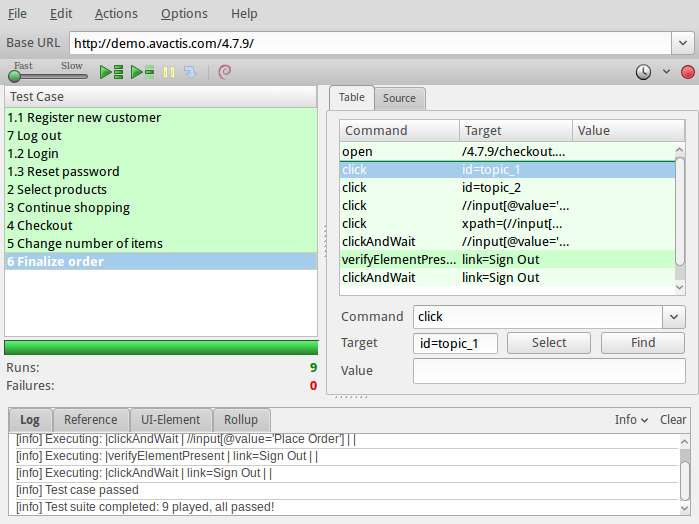
\includegraphics{TestSuitePassed}


\end{document}
